\documentclass[tikz, margin=5mm]{standalone}
\usepackage[sfdefault,light]{roboto}
\usetikzlibrary{shapes, arrows, positioning, backgrounds}
\definecolor{MyGreen}{HTML}{41B3A3}
\definecolor{MyOrange}{HTML}{E27D60}
\tikzset{every picture/.style={/utils/exec={\sffamily}}}
\begin{document}
    \begin{tikzpicture} [
			every node/.style={align=center,rectangle},
			server/.style={draw,fill=MyOrange!20,minimum width=30mm,minimum height=40mm,rounded corners},
			server_composant/.style={draw,fill=MyGreen!60,minimum width=18mm,minimum height=9mm},
			bdd/.style={draw,cylinder,shape border rotate=90,aspect=0.7,minimum width=10mm,minimum height=10mm, cylinder uses custom fill,cylinder body fill=MyGreen!60,cylinder end fill=MyGreen!20},
			legend/.style={fill=none,align=center}
		]
			\node at (-2,-0.5) [legend] (client) {
				Client \\[2ex]
				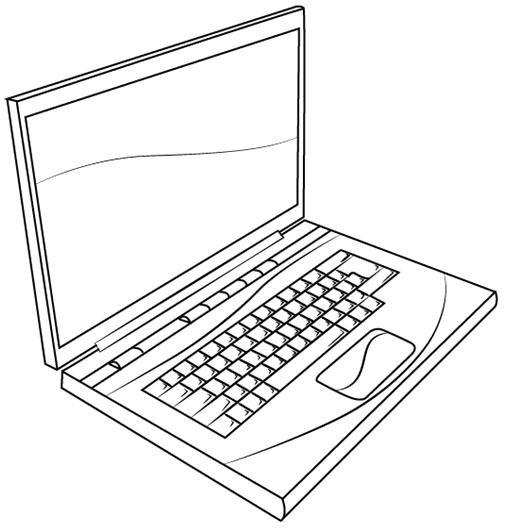
\includegraphics[width=18mm]{./images/pc.png}
			};
			\node at (4,-1) [server] (servHTTP) {};	
			\node at (4,1.7) [legend] (servName1) {Conteneur \\ Web};		
			\node at (8,-1) [server] (servMetier) {};
			\node at (8,1.7) [legend] (servName2) {Conteneur \\ Métier};
			\node at (11,-1) [bdd] (bdd) {};
			\node at (11,1.7) [legend] (servName4) {Données};
			
			\node at (4,-0.2) [server_composant] (controller) {Controleur};
			\node at (4,-1.8) [server_composant] (view) {Vue};
			\node at (8,-1) [server_composant] (model) {Modèle};
			
			\path[<->,draw,thick] (controller.east) -| (model.north);
			\path[<-,draw,dashed,thick] (view.east) -| (model.south);
			\path[->,draw,thick] (client) -- (controller);
			\path[<-,draw,thick] (client) -- (view);
			\path[<->,draw,thick] (model) -- (bdd);
			\path[->,draw,thick] (controller) -- (view);
		\end{tikzpicture}
\end{document}